\chapter{Subsystem: Operator Control and User Interface}

\section{User-Interface Design} The existing user interface uses a large black-box with a joystick, a series of buttons and switches, and a small LED display.  The box provides all major functionality that an operator could need to interface with the vehicle.  An operator can throttle, break, steer, change gears and force the vehicle to an emergency stop all from the box.  This box; however, is not the best solution for our design.

Our design requires displaying a large amount of data to an operator.  The small LED display on the box will not work for this goal.  The black-box is also not desirable because it is hard to extend.  There are a finite number of button and switches, many of which have already been programmed for essential functionality.  Our design needs a user-interface that is:
\begin{itemize}
	\item easy to use
    \item can handle displaying large amounts of information to the operator but does not overwhelm them with the info
    \item can be extended to provide extra functionality in the future 
    \item can display the most critical information in a single page view
    \ldots
\end{itemize}
  
Given these requirements, we have decided to implement a web-based user-interface.  Operators will interact with the vehicle through a web-page.  This web-page will display the incoming information from the sensor packages on the vehicle and incoming information about the state of the vehicle itself.  Most operators should be familiar with how to navigate a web-page from interacting with them on a regular basis on their own, so the interface should feel intuitive and natural to most operators.  There is also a vast amount of research on how to develop friendly and easy-to-use web-pages that our team can leverage when implementing our web-based user-interface.

\section{RobotWebTools and the ROS Control Center}Initially our team thought about replacing the black-box entirely and allow user's to drive the vehicle by using a gamepad controller.  Google Chrome and Mozilla Firefox both natively support gamepad interactions via the Gamepad API; however, we abandoned this goal to focus more on visualizing the incoming sensor data.  The black-box already contains the functionality for driving the vehicle and the Gamepad API is still in active development and is not at a state where we would feel comfortable using it for driving a vehicle.

After a large amount of research on how to visualize ROS data via a web-page we discovered the RobotWebTools group \cite{robotwebtools}. This group was actively developing tools for connecting to ROS from a website.  The architecture works by running a webserver with ROS, and then having HTML pages connect to that webserver via JavaScript.  The JavaScript library is meant to replicate the ROS architecture.  It subscribes to nodes, and when that node publishes an event, the webserver captures it, converts it into a JSON object, and then sends that object to the JavaScript library.  The JavaScript library is then free to work with that data.

The RobotWebTools provide the low end infrastructure for building a web-based user-interface with ROS.  We started to design our user-interface to be a single page view of the state of the vehicle and visualize all of the sensor data.  We decided on this because a user needs to be able to focus on driving the vehicle, and forcing them to have to click through tabs to find the data that they needed seemed unreasonable.  The sheer amount of data that we are processing makes this difficult.  We have a handful of sensors and cameras, the LIDAR, and vehicle state and location data to display in one page.  Furthermore, we need our interface to be flexible and dynamic so that it can subscribe to all of the necessary nodes immediately without needing to be reconfigured.  If we add new nodes for new sensors on the vehicle, then we want our user-interface to be able to identify and display that data with little effort.

While researching how to accomplish our user-interface, we discovered that someone else had recently publicly posted a web-based user-interface that was built on top of the RobotWebTools libraries.  The project is called the ROS Control Center and is an AngluarJS project which provides a template for how to build a web-based user-interface to visualize ROS data \cite{roscontrolcenter}.

\begin{figure}[H]
\centerline{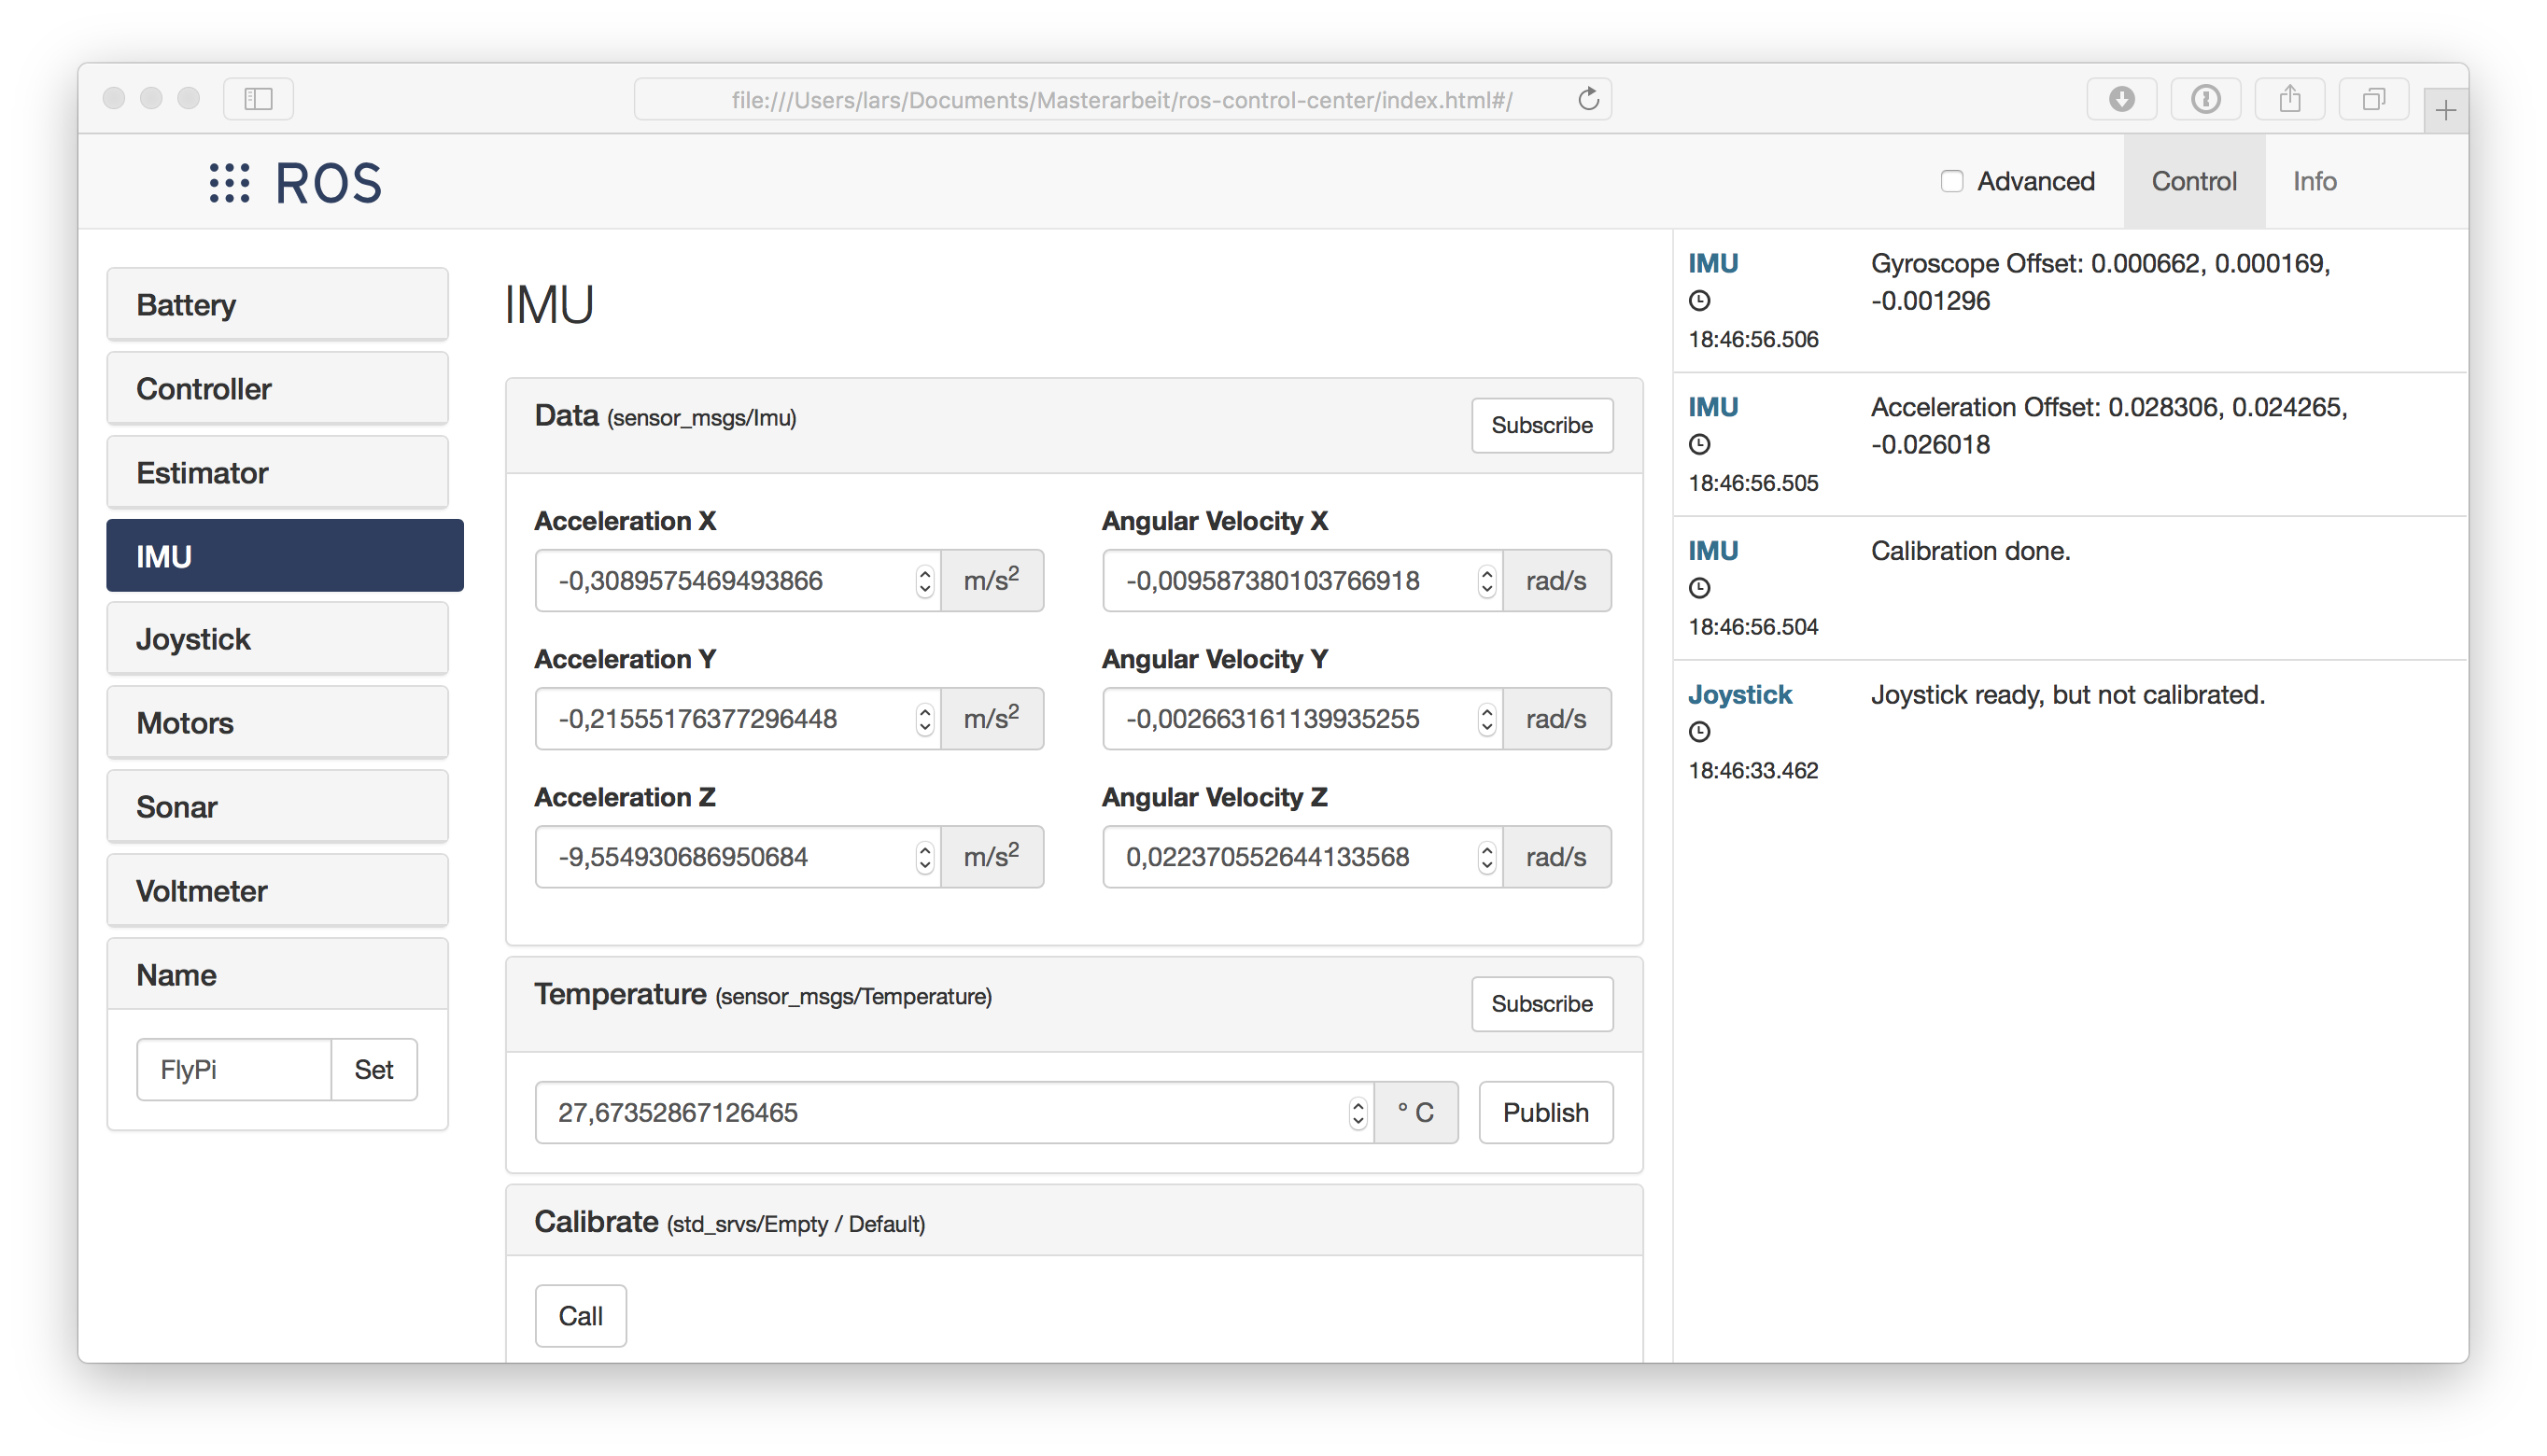
\includegraphics[angle=0,width=1\linewidth]{ros_control_center_screenshot}}
\caption[]{ROS Control Center}
\label{fig:roscontrolcenter}
\end{figure}

As seen in \ref{fig:roscontrolcenter}, the ROS Control center comes prepackaged with visualization for a variety of default ROS packages, but these visualizations are limited to text displays of incoming data.  The ROS Control Center works by asking the RobotWebTools web server for all nodes that are currently publishing messages.  These node, message type pairings create unique names as part of the ROS architecture.  The ROS Control Center leverages this feature and creates an associative array where each node is a key and each value is the message type.  When the ROS Control Center recognizes a node, it adds the node to the left-side navigation bar.  Then, the ROS Control Center embeds the HTML code for visualizing the individual message types into the page.  This way, a user can click on a particular node's name, and then see all of data for all of the messages that belong to that node.  Writing these HTML files for each message is fairly simple to do because the ROS Control Center handles all of the data processing.

The ROS Control Center is not a perfect solution.  It does not provide a one page view of the vehicle's most critical systems.  It also does not come pre-packaged with any graphing ability.  The ROS Control Center also does not provide any way to handle the idea of thresholds and warnings. Many of the environmental hazards we are trying to detect have safe and unsafe thresholds.  We want our user-interface to be able to provide feedback to the user when the unsafe thresholds are exceeded to quickly alert the user that there is a problem.

These are all features that can be added to the ROS Control Center.  Since each message is given it's own HTML page, we can write the JavaScript logic in those pages to handle alerts for safe and unsafe conditions and build live-stream plots in those pages too.  We can also build a page that uses the data from multiple messages and displays them in one page.  Adding these features on top of the ROS Control Center will meet our design requirements and goals.

\section{Improving the ROS Control Center}
We made several breaking changes to the ROS Control Center in order to implement the features that we wanted to.  The largest issue with the ROS Control Center framework is that it doesn't provide any easy way to display data from multiple nodes in one page.  In order to implement this feature we force the ROS Control Center to load a fake \"Dashboard\" topic.  This topic is always the first one to load and display and subscribes to the different topics that we need it to.  Currently the Dashboard topic subscribes to the three different environmental sensor packages, the LIDAR point cloud, the four cameras, and the vehicle state information.  Not all of the data from each message is displayed on this page.  Instead we identified what we believe to be the most critical parts of each topic.  

[INSERT IMAGE OF UI]

On the left side of the screen are the camera feeds - front, right, left and rear.  In the center of the page is the visualization of the LIDAR point cloud using the \url{https://github.com/RobotWebTools/ros3djs}<ros3djs> library provided by the RobotWebTools.  Part of that LIDAR visualization also includes rendering the model of the rover within the cloud.  The reason that the point cloud is the prominent feature on the page is that the cameras don't always provide the most reliable view of the environment.  Factors such as smoke will make it difficult for an operator to drive the vehicle while using the cameras.  The LIDAR point cloud however will always generate a reliable scan of the environment and give operators a clear view of where the vehicle is.  The right side of the page is a combination of the vehicle state information (the speed of the vehicle) and the environmental sensors.

All of the charts are created using the \url{https://github.com/pablojim/highcharts-ng}<highcharts-ng> AngularJS library which provides a convenient way to use \url{http://www.highcharts.com/}<Highcharts> in AngularJS.

\subsection{Rendering the LIDAR Point Cloud}
Rendering the LIDAR point cloud presented a special challenge.  The data coming off of the LIDAR is simply a line of what the LIDAR is scanning.  As the LIDAR moves up and down it publishes these lines, and it is then the responsibility of the visualizing software to aggregate these lines and display the resulting cloud.

There are two potential solutions to this problem:
\begin{enumerate}
    \item Assign each point a timer, and when the timer expires, remove the point
    \item Only hold so many points in the scene at once
\end{enumerate}

For our implementation, we chose to only hold so many points on the screen at once.  The ros3djs library allows you to set a maximum number of points that you can display on the screen, but it assumes that you are already giving it a full point cloud.  We went add added the ability to have the scene aggregate the points during render time.  Essentially, we keep track of the last index that we wrote points to, and on the next message, we start writing at that location.  When we reach the end of the array, we start back the beginning and overwrite old points with new information.  We currently have the scene set to hold 75,000 points at once, which seems to hold about three to five seconds worth of point cloud data, which is plenty of time to visualize the surrounding environment as the vehicle moves through it.

We also need to assign color to the points.  If we didn't assign colors, the entire cloud would be gray which can makes it hard to distinguish what's in the cloud.  We use a quick linear-interpolation to determine color of a given point by using its y-axis value.  We chose the y-axis value because it gave us the best clarity.  The colors progress from red to green to blue as you move upward in the scene.  This interpolation isn't perfect though.  It actually cycles through the color wheel before reaching the max y-axis value.  This was done partially on purpose to provide greater clarity.  Our first attempt at coloring the scene made people hard to distinguish.  A standing body takes up a very small portion of y-axis values, and so they were appearing as single colored blobs.  We allowed the colors to cycle in order to allow small objects to be more visible; however, we may have allowed the colors to cycle too much.  Now, there are almost too many colors on the screen which can make it hard to process.


\section{Network for Internet Communication}The RobotWebTools libraries and the ROS Controller Center assume that there is an internet connection between ROS and the device running the ROS Controller Center.  The rover is meant to be deployed in rugged, off-road terrain where an existing internet connection is not necessarily available.  To deal with this problem, we purchased a high-power router that sits on the vehicle.  On the vehicle we run the RobotWebTools rosbridge\char`_server package and a small HTTP web-server.  The rosbridge\char`_server package handles translating ROS messages to a JSON format so that the web-client can use the data.

\begin{figure}[H]
\centerline{\includegraphics[angle=0,width=1\linewidth]{NetworkRover}}
\caption[]{Network architecture to enable the user-interface}
\label{fig:NetworkRover}
\end{figure}

Ideally, we would want the rover to be able to serve up the HTML pages and JavaScript files necessary to run the UI.  Unfortunately, all of the computer systems currently on the rover are already overburdened.  Our current solution is to just download our modified version of the ROS Control Center on a laptop and then load the page from a browser locally.  This has worked well enough for our use cases, although in the future, it would be nice to have the vehicle serve the files.  This would require the least amount of setup for accessing the user interface in the field.